\section{Проектирование программного средства}

Исходя из требований и современных стандартов разработки, программное средство должно обладать следующими свойствами:
\begin{itemize}
    \item модульность;
    \item простота горизонтального масштабирования;
    \item параллельная обработка данных;
    \item безопасность хранения конфиденциальных и личных данных.
\end{itemize}

Для соответствия выше описанным свойствам было принято решение разрабатывать программное средство в виде изолированных модулей и использовать архитектуру микросервисов. Так как использование монолитной архитектуры затруднит горизонтальное масштабирование и увеличит связность модулей, что усложнит последующее сопровождение. 

Разработанное программное средство состоит из следующих модулей, рисунок~\ref{fig:architecture:deployment}:
\begin{itemize}
    \item модуль выделения признаков почерка;
    \item модуль определения параметров личности;
    \item модуль биометрической аутентификации;
    \item модуль определения неврологических отклонений;
    \item модуль контроля доступа;
    \item модуль управление образцами почерка;
    \item модуль доступа к базе данных.
\end{itemize}

Вышеописанные модули опираются на следующие группы классов, разработанные в рамках диссертационной работы:
\begin{itemize}
    \item Набор классов для сегментации образца на строки, слова, символы и выделения признаков. Написан на языке Scala.
    \item Набор классов машинного обучения (для классификации признаков текста). Написан на языке программирования Scala и содержит реализацию алгоритма основанного на методе опорных векторов (Support Vector Machine), подробнее рассмотрен в главе~\ref{sec:architecture:personal_parameters}.
    \item Набор классов для контроля доступа. Написана на языке Scala. Содержит классы для регистрации, авторизации и управлением сессией пользователя. Основан на стандарте JSON Web Token (JWT).
    \item Набор классов для организации доступа и хранения авторизационных данным пользователя и коллекции обработанных образцов.
\end{itemize}

Далее приведено подробное описание структуры и назначения каждого модуля.

\afterpage{
  \todo[inline]{Обновить}
  \begin{figure}[t!]
  \centering
    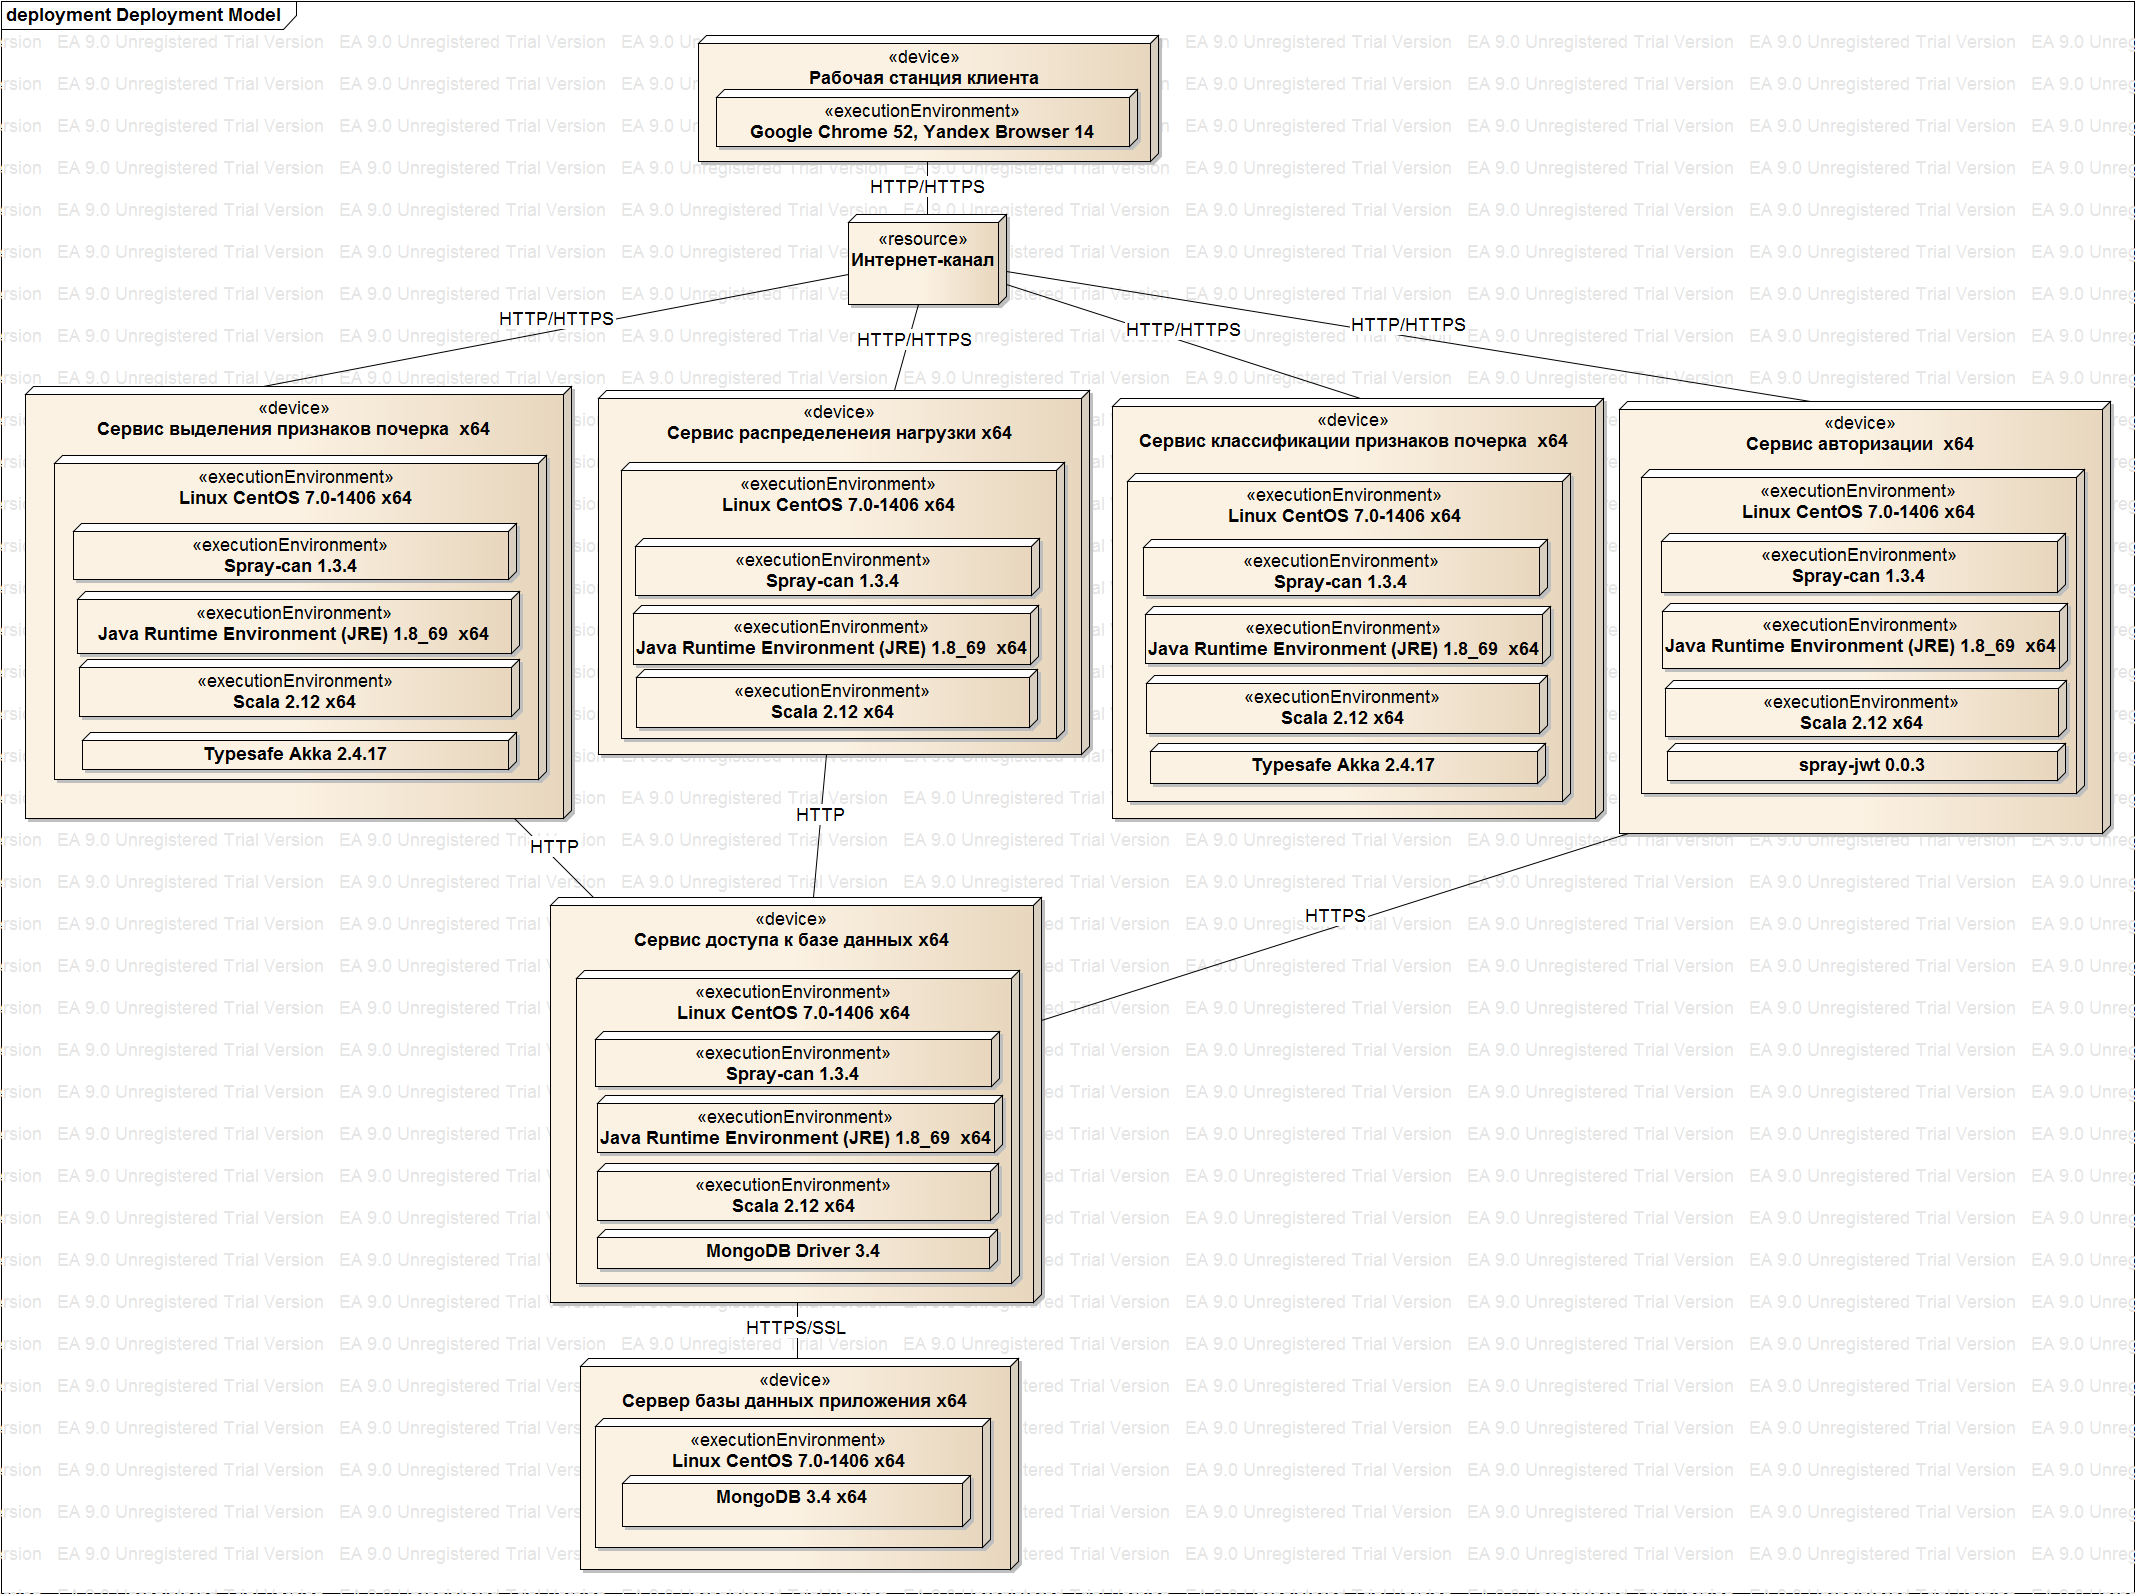
\includegraphics[scale=0.52]{figures/deployment_model.png}
    \caption{Диаграмма развертывания программного средства}
    \label{fig:architecture:deployment}
  \end{figure}
}
\todo[inline]{Модуль аутентификации, строит Гаусовское распределение параметров и сопостовляет с эталоном}
\todo[inline]{Модуль микрографии, делает скелетизацию и СКО}
\subsection{Модуль определения параметров личности}
\label{sec:architecture:personal_parameters}
Основываясь на анализе литературных источников в разделе~\ref{sub:domain:literary_sources} и спецификации требований, раздел~\ref{sec:freq:psiho_analysis}, было принято решение для определения параметров личности по признаком рукописного текста использовать классификатор на основе метода опорных векторов, широко используемого метода машинного обучения~\cite{manning_ir}, который при своей относительной простоте реализации, позволяет добиться очень неплохих результатов классификации.

Метод опорных векторов (\emph{SVM, support vector machine}) – семейство схожих алгоритмов обучения с учителем, использующихся для задач классификации и регрессионного анализа. Особым свойством метода опорных векторов является непрерывное уменьшение эмпирической ошибки классификации и увеличение зазора, поэтому метод также известен как метод классификатора с максимальным зазором~\cite{mitchell_ml, wiki_SVM}.

Параметры текста представляют собой непрерывные величины подчиняющиеся нормальному распределению, рисунок~\ref{fig:architecture:normal_pd}. Исходя их этого свойства использование полиномиальных однородных и неоднородных ядер не позволит достичь хороший результатов классификации, для достижения хороших результатов распознавания следует использовать в качестве ядер радиально-базисная функцию Гаусса~\cite{wiki_gauss, orr}, формула~(\ref{eq:architecture:gaussian_core}).

\begin{equation}
  \label{eq:architecture:gaussian_core}
  k(x, x^{'}) = \exp(-\frac{\left|\left| x - x^{'} \right|\right|}{2\sigma_{}^2})
\end{equation}
\begin{explanation}
где & $x^{'}$ & среднее значение параметра, рассчитанное для объектов, принадлежащих
классу $C$; \\
    & $ \sigma_{}^2 $ & дисперсия значения параметра объектов из класс $C$.
\end{explanation}

Дисперсия значения параметра представлена формулой~(\ref{eq:architecture:dispersion}).
\begin{equation}
  \label{eq:architecture:dispersion}
  \sigma_{}^2 = \frac{1}{n - 1} \sum\limits_{x \in C} (x_i - \overline{x_{}}^2)
\end{equation}

\begin{figure}[!h]
    \centering
    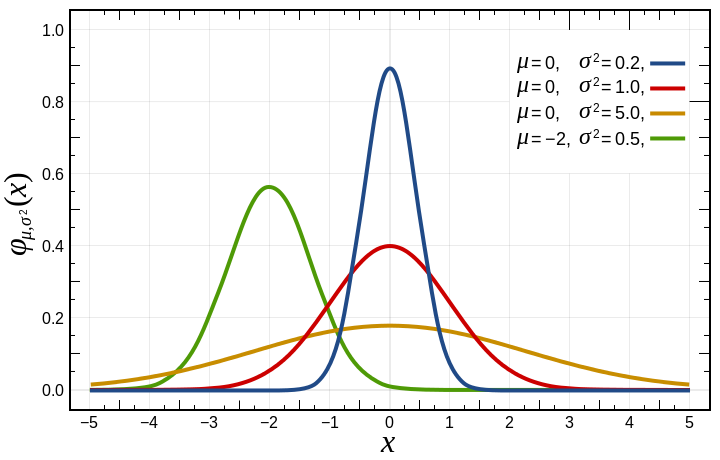
\includegraphics[width=0.85\textwidth]{figures/gauss.png}
    \caption{График функции плотности вероятности для нормального распределения}
    \label{fig:architecture:normal_pd}
\end{figure}

\subsection{Модуль выделения признаков почерка}
На основании требование сформированных в разделе~\ref{sec:freq:extract_features} основным функциями данного модуля является:
\begin{itemize}
  \item подготовка образца к обработке;
  \item сегментация образца;
  \item выделения признаков почерка.
\end{itemize}

Учитывая цифровой формат ввода образца, процесс подготовки сводится к построению единной матрицы координат точек из двух массивов координат точек и массива флагов разрыва.

Следующий этапам является сегментация образца, а первой стадией сегментации является сегментация строк.
Задача выделения строк сводиться к нахождению верхних и нижних граней строк текста на исходном образце. Алгоритм сегментации строк основывается на том, что средняя плотность точек в межстрочных промежутках существенно ниже средней плотности точек в текстовых строк~\cite{cv_text_image_segmentator}.

Первым этапом необходимо для всех строк образца находим их значения плотности точек, формула~(\ref{eq:architecture:line_medium_brigth}).
\begin{equation}
  \label{eq:architecture:line_medium_brigth}
  d_j = d_j(M) = \frac{1}{n}\cdot\sum\limits_{i=1}^{n} m_{ij}
\end{equation}

Затем необходимо определить среднюю плотность точек всего образца, \mbox{формула~(\ref{eq:architecture:medium_brigth}).}
\begin{equation}
  \label{eq:architecture:medium_brigth}
  d(M) = \frac{1}{l}\cdot\sum\limits_{j=1}^{l} d_j(M)
\end{equation}

Средняя плотность точек в межстрочных интервалах невелика (близка к нулю). Поэтому плотность точек верхней границы строки можно выразить из плотности точек всего образца, формула~(\ref{eq:architecture:line_up_interval_medium_brigth}).
\begin{equation}
  \label{eq:architecture:line_up_interval_medium_brigth}
  d^{t} = k_{t} \cdot d(M)
\end{equation}
\begin{explanation}
где & $ k_{t} $ & коэффициент от 0 до 1
\end{explanation}

Аналогично плотность нижней границы может быть выражена через плотности точек всего образца, формула~(\ref{eq:architecture:line_down_interval_medium_brigth}).
\begin{equation}
  \label{eq:architecture:line_down_interval_medium_brigth}
  d^{b} = k_{b} \cdot d(B)
\end{equation}
\begin{explanation}
где & $ k_{b} $ & коэффициент от 0 до 1
\end{explanation}

Работа алгоритма заключается в последовательном просмотре массива средних значений $ (d_1,...,d_m) $ и выявлении множества пар индексов $ (d^t_i,d^b_i) $ строк соответствующих ниже приведенным условиям и следовательно являющимися верхней $ d^t_i $ и нижней $ d^b_i $ границам строк.

Условия верхней границы текстовой строки:
\begin{itemize}
  \item плотность точек текущей строки превышает границу $ d^{t} $;
  \item плотность точек двух предыдущих строк ниже этой границы;
  \item плотность точек трех последующих строк выше границы $ d^{b} $.
\end{itemize}

Следовательно должно выполняться логическое условие описанное формулой~(\ref{eq:architecture:logic_up_interval}).
\begin{equation}
  \label{eq:architecture:logic_up_interval}
  (d_{i-2} < d^{t}) \wedge (d_{i-1} < d^{t}) \wedge (d_i > d^{b}) \wedge (d_{i+1} > d^{b}) \wedge (d_{i+2} > d^{b}) \wedge (d_{i+3} > d^{b})
\end{equation}

Условия нижней границы текстовой строки:
\begin{itemize}     
  \item было зафиксировано начало области;
  \item плотность точек текущей строки превышает границу $ d^{t} $;
  \item плотность точек последующей строки ниже границы $ d^{b} $.
\end{itemize}
     
Или:

\begin{itemize}
   \item было зафиксировано начало области;
   \item плотность точек трех последующих строк ниже границы $ d^{b} $.
\end{itemize}

Следовательно должно выполняться логическое условие описанное формулой~(\ref{eq:architecture:logic_down_interval}).
\begin{equation}
  \label{eq:architecture:logic_down_interval}
  ((d_{i+1} < d^{b}) \wedge (d_{i+2} < d^{b}) \wedge (d_{i+3} < d^{b}) \vee ((d_i > d^{t}) \wedge (d_{i+1} < d^{b})))
\end{equation}

Результатом работы алгоритма является множество пар индексов верхних и нижних границ строк. На основе этих данных можно рассчитать высоты строки (разность между индексами). Недостатком данного алгоритма является <<срезание>> символов, которые имеют высоту выше средней.

Для устранения этого недостатка можно использовать следующий прием расширения найденной границы. Необходимо определить строку с минимальной высотой $ H_{min} $, а затем границы всех строк на величину $ 0.3 \cdot  H_{min} $. Данный шаг не приведет к слиянию строк, т.к. межстрочные интервалы текста, как правило, больше чем высота строки.
 
Алгоритмы сегментации слов и символом сходи с алгоритмом сегментации строк. Основными отличиями являются необходимость построения карты плотности столбцов, а не строк, а так же наличие дополнительных этапов постобработки, направленных на удаление ложных границ после сегментации слов и символов. Исходными данными следующего алгоритма являются результаты работы предыдущего, так на вход алгоритма сегментации слов подается результат сегментации строк.

Так же для сегментации образцов можно использовать готовый алгоритм реализованный в сторонней системы распознавания рукописного текста, например Tesseract или ABBYY FineReader. Однако данный подход требует дополнительных усилий по предварительной обработке образца почерка и лишает разработчика возможности оптимизировать алгоритм под конкретную задачу. Помимо часть подобных средств распространяется на платной основе, что увеличит стоимость разработки и сопровождения.

Следующей функцией данного модуля является выделение из образца следующих признаков текста:
\todo[inline]{Рассширить список параметров} 
\begin{itemize}
  \item наклон символов;
  \item наклон строк;
  \item интервал между символами;
  \item интервал между словами;
  \item интервал между строками;
  \item частота текста.
\end{itemize}

Для определения угла наклона символа необходимо определить координаты верхней и нижней точек символа и используя арктангенс вычислить угол, формула~(\ref{eq:architecture:symbol_angle}).

\begin{equation}
  \label{eq:architecture:symbol_angle}
  \Theta = \tan^{-1}{\frac{y_2 - y_1}{x_2 - x_1}}
\end{equation}
где  $\Theta$ - угол наклона символа \\
     $ (x_1, y_1) (x_2, y_2) $  - координаты крайних точек символа.


\begin{figure}[ht]
    \centering
    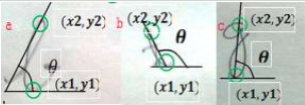
\includegraphics[width=0.85\textwidth]{figures/char_angle.png}
    \caption{Пример расчета угла наклона символа}
    \label{fig:architecture:symbol_angle}
\end{figure}

На изображении~\ref{fig:architecture:symbol_angle} приведены примеры символов с выделенными верхними и нижними точками, координаты $ (x_2, y_2) и (x_1, y_1) $ соответственно и условно обозначенным угол $ \Theta $. Представлены образцы трех типов наклона символов левосторонний, правосторонний и прямой.

Сегментация рукописного текста является нетривиальной задачей ввиду непостоянства таких параметров как пробелы между символами, в плодь до их отсутствия, словами и строками. Задача становится еще сложнее учитывая то, что данные признаки необходимо сохранить и использовать в дальнейшей работе.

\todo[inline]{Вычитать}
Поскольку процесс сегментации образцов и выделение признаков являются относительно долгими операциями, сегментация вместе с выделением признаков занимает от 0.5 до 1 секунды, в зависимости от особенностей образца, обеспечение параллельной обработки выходит на передний план. К счастью выбранные признаки почерка независимы и могут рассчитываться параллельно. Так же нет необходимость ожидать полной сегментации сегментации для начала выделения признаков, например интервал между строками можно вычислить сразу после разбиения образца на строки. Это позволит значительно ускорить работу данного модуля.

\subsection{Модуль доступа к данным}
Данный модуль отвечает за организацию работы с базой данных и предоставление другим модулям удобного интерфейса.
На основании требований сформированных в разделах~\ref{sec:freq:show},~\ref{sec:freq:add},~\ref{sec:freq:delete}, основными функциями данного модуля являются:
\begin{itemize}
  \item добавление авторизационных данных пользователя в базу при регистрации (включая проверку дублирования имен пользователей);
  \item проверка наличия пользователя в базе и соответствие хеша пароля;
  \item добавление нового образца в базу;
  \item обновление информации о параметрах образца;
  \item удаление образца из базы.
\end{itemize}

Так как список параметров образца постоянный и параметры рассчитываются и обновляются параллельно, в данном случае рационально использование классической реляционной базы данных, в тоже время на базу данных не налагается каких-либо существенных ограничений по быстродействию и скорости обработки запросов. Основываясь на выше перечисленном в качестве СУБД была выбрана PosgreSQL.
Так же плюсом этого решения можно отнести хранение документов в базе в виде JSON-объектов, что исключает дополнительное преобразование данных перед отправкой их другим сервисам и на клиент, а так же отсутствие платы за использование, что позволит снизить стоимость разработки и использования.

\subsection{Модуль контроля доступа}
Поскольку разрабатываемое приложение может содержать персональные данные пользователя, вплоть до имени и фамилии в графе комментариев к образцу, задача организации безопасного доступа и хранению подобных данных стоит довольно остро.
Данный модуль отвечает за регистрацию и авторизацию пользователей. 
В данной работе для предоставления защищенного доступа к модулям будет использоваться открытый стандарт JSON Web Token (RFC 7519). JWT-маркер  содержит в зашифрованном виде всю минимально необходимую информацию для аутентификации и авторизации. При этом не требуется хранить в сессии данных о пользователе, так как маркер самодостаточный. Данный факт упрощает горизонтальное масштабирование системы и хорошо подход для архитектур на основе микросервисов.

На основании требований, сформированных в разделах~\ref{sec:freq:reg} и~\ref{sec:freq:auth}, основными функциями данного модуля являются:
\begin{itemize}
  \item регистрации новых пользователей;
  \item авторизация пользователей;
  \item генерация JWT"=маркеров.
\end{itemize}

\begin{figure}[ht]
    \centering
    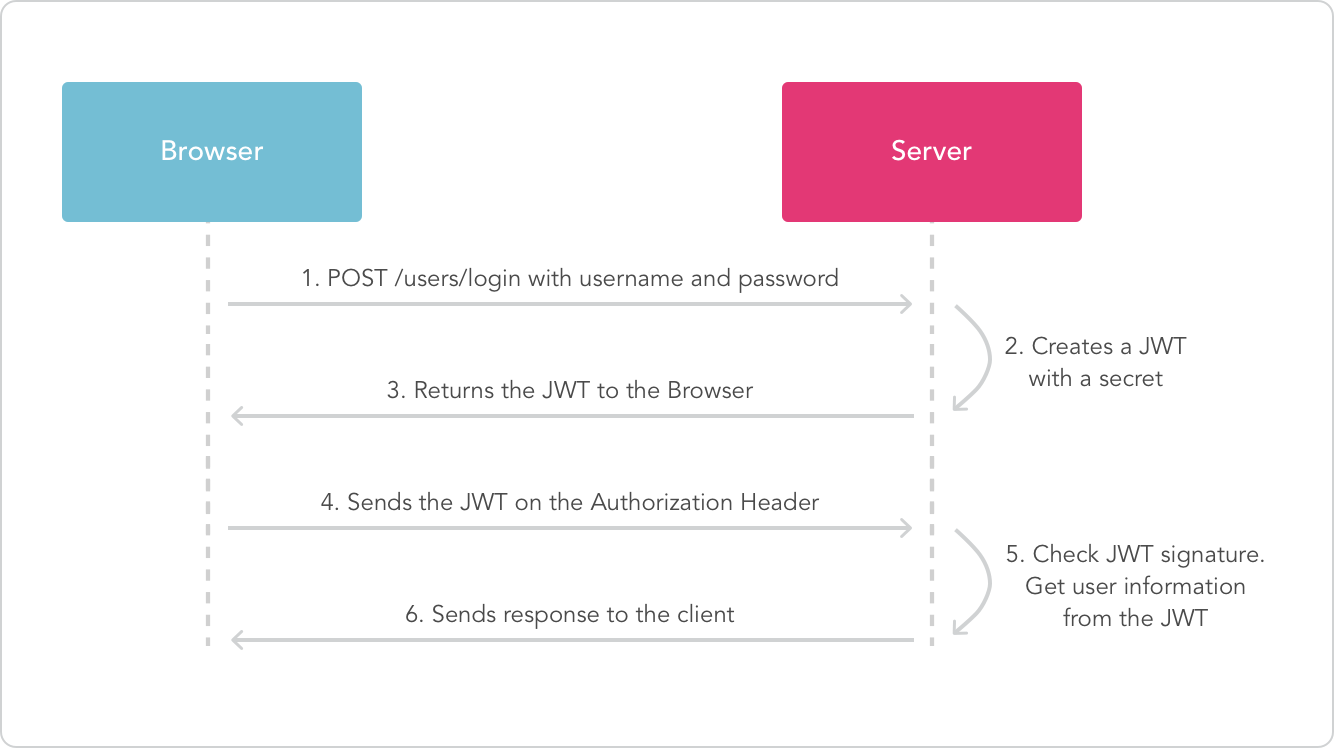
\includegraphics[width=0.7\textwidth]{figures/jwt_diagram.png}
    \caption{Диаграмма генерации и верификации JWT-маркеров}
    \label{fig:architecture:jwt_diagram}
\end{figure}

На рисунке~\ref{fig:architecture:jwt_diagram} представлен алгоритм создания, подписи и проверки JWT-маркера. В данном примере выдачу и проверку маркера осуществляет один и тот же сервер, однако, как было описано выше, это не является обязательным условием и представлено лишь для упрощения диаграммы.

Использование контроля доступа на основе JWT-маркеров позволяет снизить нагрузку на сервис контроля доступа, благодаря возможности проверки подлинности маркера на стороне других сервисов.